%%%%%%%%%%%%%%%%%%%%%%%%%%%%%%%%%%%%%%%%%
% Bachelor/Master-Arbeit
% Vorlage HTWG EI
%
% Basierend auf
% 
% LaTeX Template
% Version 2.5 (27/8/17)
%
% This template was downloaded from:
% http://www.LaTeXTemplates.com
%
% Version 2.x major modifications by:
% Vel (vel@latextemplates.com)
%
% This template is based on a template by:
% Steve Gunn (http://users.ecs.soton.ac.uk/srg/softwaretools/document/templates/)
% Sunil Patel (http://www.sunilpatel.co.uk/thesis-template/)
%
% Template license:
% CC BY-NC-SA 3.0 (http://creativecommons.org/licenses/by-nc-sa/3.0/)
%
%%%%%%%%%%%%%%%%%%%%%%%%%%%%%%%%%%%%%%%%%

%----------------------------------------------------------------------------------------
%	PACKAGES AND OTHER DOCUMENT CONFIGURATIONS
%----------------------------------------------------------------------------------------

\documentclass[
11pt, % The default document font size, options: 10pt, 11pt, 12pt
%oneside, % Two side (alternating margins) for binding by default, uncomment to switch to one side
ngerman, % english for English
singlespacing, % Single line spacing, alternatives: onehalfspacing or doublespacing
%draft, % Uncomment to enable draft mode (no pictures, no links, overfull hboxes indicated)
%nolistspacing, % If the document is onehalfspacing or doublespacing, uncomment this to set spacing in lists to single
%liststotoc, % Uncomment to add the list of figures/tables/etc to the table of contents
%toctotoc, % Uncomment to add the main table of contents to the table of contents
%parskip, % Uncomment to add space between paragraphs
%nohyperref, % Uncomment to not load the hyperref package
headsepline, % Uncomment to get a line under the header
%chapterinoneline, % Uncomment to place the chapter title next to the number on one line
%consistentlayout, % Uncomment to change the layout of the declaration, abstract and acknowledgements pages to match the default layout
]{MastersDoctoralThesis} % The class file specifying the document structure

\usepackage[utf8]{inputenc} % Required for inputting international characters
\usepackage[T1]{fontenc} % Output font encoding for international characters

\usepackage{mathpazo} % Use the Palatino font by default

\usepackage[backend=bibtex,style=ieee-alphabetic, bibstyle=ieee-alphabetic, maxnames=3,minnames=1,natbib=true]{biblatex} % Use the bibtex backend with the authoryear citation style (which resembles APA)

\addbibresource{example.bib} % The filename of the bibliography

\usepackage[autostyle=true]{csquotes} % Required to generate language-dependent quotes in the bibliography

%----------------------------------------------------------------------------------------
%	MARGIN SETTINGS
%----------------------------------------------------------------------------------------

\geometry{
	paper=a4paper, % Change to letterpaper for US letter
	inner=2.5cm, % Inner margin
	outer=3.8cm, % Outer margin
	bindingoffset=.5cm, % Binding offset
	top=1.5cm, % Top margin
	bottom=1.5cm, % Bottom margin
	%showframe, % Uncomment to show how the type block is set on the page
}

%----------------------------------------------------------------------------------------
%	THESIS INFORMATION
%----------------------------------------------------------------------------------------

\thesistitle{Entwicklung einer KI-basierten Spurerkennung als externe Sensorik} % Todo: Titel aus EI-Portal

\thesistitle{Kamerabasierte Lane-Detection, als Grundlage zur Bewertung von Spurmittenführung/Spurverlassensverhinderung} % Todo: Titel aus EI-Portal
\supervisor{Prof.~Dr.-Ing Christopher Knievel} % Your supervisor's name, this is used in the title page, print it elsewhere with \supname
\supervisors{Dipl. Math. Tom Wagemann}
\examiner{} % Your examiner's name, this is not currently used anywhere in the template, print it elsewhere with \examname
\company{Audi AG} % Name der Firma
\degree{Bachelor of Engineering} % Your degree name, this is used in the title page and abstract, print it elsewhere with \degreename
\author{Tim \textsc{Alkofer}} % Your name, this is used in the title page and abstract, print it elsewhere with \authorname
\addresses{} % Your address, this is not currently used anywhere in the template, print it elsewhere with \addressname

\subject{} % Your subject area, this is not currently used anywhere in the template, print it elsewhere with \subjectname
\keywords{} % Keywords for your thesis, this is not currently used anywhere in the template, print it elsewhere with \keywordnames
\university{Hochschule Konstanz - Technik, Wirtschaft und Gestaltung} % Your university's name and URL, this is used in the title page and abstract, print it elsewhere with \univname

\AtBeginDocument{
\hypersetup{pdftitle=\ttitle} % Set the PDF's title to your title
\hypersetup{pdfauthor=\authorname} % Set the PDF's author to your name
\hypersetup{pdfkeywords=\keywordnames} % Set the PDF's keywords to your keywords
}

\begin{document}

\frontmatter % Use roman page numbering style (i, ii, iii, iv...) for the pre-content pages

\pagestyle{plain} % Default to the plain heading style until the thesis style is called for the body content

%----------------------------------------------------------------------------------------
%	TITLE PAGE
%----------------------------------------------------------------------------------------

\begin{titlepage}
\begin{center}

  \vspace*{.06\textheight}
  \begin{minipage}[t]{\textwidth}
    
\includegraphics[width=0.4\textwidth, keepaspectratio]{Figures/htwg.png}\hspace{0.19\textwidth} 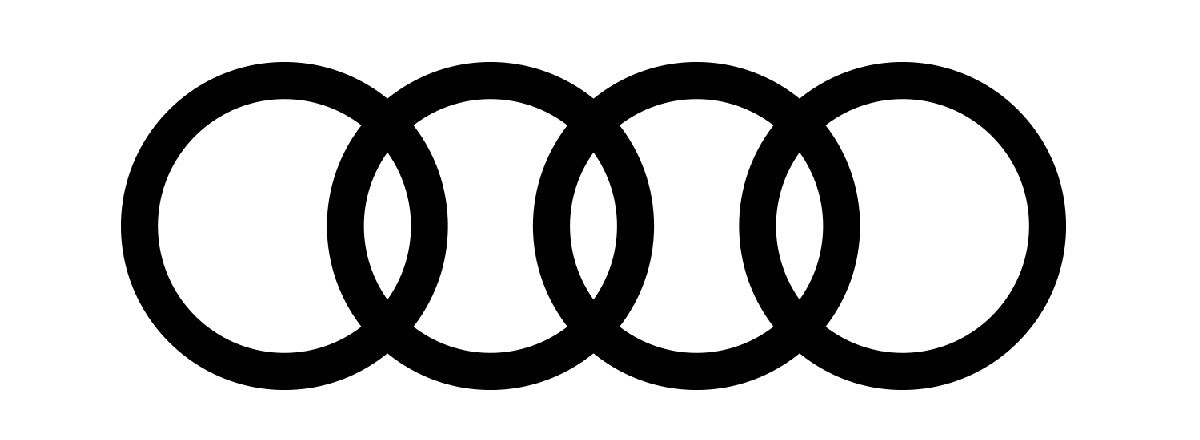
\includegraphics[width=0.4\textwidth,keepaspectratio]{Figures/AL090142_large.jpg}
  \end{minipage}
  {\scshape\LARGE \univname\par\vspace{1em}\supcompany}\vspace{1.5cm} % University name

\HRule \\[0.4cm] % Horizontal line
{\huge \bfseries \ttitle\par}\vspace{0.4cm} % Thesis title
\HRule \\[1.5cm] % Horizontal line

Arbeit zur Erlangung des akademischen Grades: \\[0.4cm]
\textsc{\Large \bfseries \glqq \degreename \grqq}\\[1cm] % Thesis type
absolviert bei der  \\[0.5cm]
\textsc{\Large \bfseries \supcompany}
\\[2cm]
\begin{minipage}[t]{\textwidth}
\begin{flushleft} \large
\emph{Autor:} \authorname % Author name - remove the \href bracket to remove the link
\end{flushleft}
\end{minipage}
\\[1.0cm]
\begin{minipage}[t]{\textwidth}
\begin{flushleft} \large
\emph{1. Prüfer:}
\supname % Supervisor name - remove the \href bracket to remove the link
\\
\emph{2. Prüfer:}
\supnames \\[1cm]
\emph{Eingereicht am:} \today
\end{flushleft}
\end{minipage}\\[3cm]
 
\vfill
\end{center}
\end{titlepage}

%----------------------------------------------------------------------------------------
%	DECLARATION PAGE
%----------------------------------------------------------------------------------------

\begin{declaration}
\addchaptertocentry{\authorshipname} % Add the declaration to the table of contents
\noindent I, \authorname, declare that this thesis titled, \enquote{\ttitle} and the work presented in it are my own. I confirm that:

\begin{itemize} 
\item This work was done wholly or mainly while in candidature for a research degree at this University.
\item Where any part of this thesis has previously been submitted for a degree or any other qualification at this University or any other institution, this has been clearly stated.
\item Where I have consulted the published work of others, this is always clearly attributed.
\item Where I have quoted from the work of others, the source is always given. With the exception of such quotations, this thesis is entirely my own work.
\item I have acknowledged all main sources of help.
\item Where the thesis is based on work done by myself jointly with others, I have made clear exactly what was done by others and what I have contributed myself.\\
\end{itemize}
 
\noindent Signed:\\
\rule[0.5em]{25em}{0.5pt} % This prints a line for the signature
 
\noindent Date:\\
\rule[0.5em]{25em}{0.5pt} % This prints a line to write the date
\end{declaration}

\cleardoublepage


%----------------------------------------------------------------------------------------
%	ACKNOWLEDGEMENTS
%----------------------------------------------------------------------------------------

\begin{acknowledgements}
\addchaptertocentry{\acknowledgementname} % Add the acknowledgements to the table of contents
The acknowledgments and the people to thank go here, don't forget to include your project advisor\ldots
\end{acknowledgements}

%----------------------------------------------------------------------------------------
%	LIST OF CONTENTS/FIGURES/TABLES PAGES
%----------------------------------------------------------------------------------------

\tableofcontents % Prints the main table of contents

\listoffigures % Prints the list of figures

\listoftables % Prints the list of tables

%----------------------------------------------------------------------------------------
%	ABBREVIATIONS
% ----------------------------------------------------------------------------------------

\begin{abbreviations}{ll} % Include a list of abbreviations (a table of two columns)

\textbf{LAH} & \textbf{L}ist \textbf{A}bbreviations \textbf{H}ere\\
\textbf{WSF} & \textbf{W}hat (it) \textbf{S}tands \textbf{F}or\\

\end{abbreviations}

%----------------------------------------------------------------------------------------
%	PHYSICAL CONSTANTS/OTHER DEFINITIONS
%----------------------------------------------------------------------------------------

\begin{constants}{lr@{${}={}$}l} % The list of physical constants is a three column table

% The \SI{}{} command is provided by the siunitx package, see its documentation for instructions on how to use it

Speed of Light & $c_{0}$ & \SI{2.99792458e8}{\meter\per\second} (exact)\\
%Constant Name & $Symbol$ & $Constant Value$ with units\\

\end{constants}

%----------------------------------------------------------------------------------------
%	SYMBOLS
%----------------------------------------------------------------------------------------

\begin{symbols}{lll} % Include a list of Symbols (a three column table)

$a$ & distance & \si{\meter} \\
$P$ & power & \si{\watt} (\si{\joule\per\second}) \\
%Symbol & Name & Unit \\

\addlinespace % Gap to separate the Roman symbols from the Greek

$\omega$ & angular frequency & \si{\radian} \\

\end{symbols}

%----------------------------------------------------------------------------------------
%	DEDICATION
%----------------------------------------------------------------------------------------

\dedicatory{For/Dedicated to/To my\ldots} 

%----------------------------------------------------------------------------------------
%	THESIS CONTENT - CHAPTERS
%----------------------------------------------------------------------------------------

\mainmatter % Begin numeric (1,2,3...) page numbering

\pagestyle{thesis} % Return the page headers back to the "thesis" style

% Include the chapters of the thesis as separate files from the Chapters folder
% Uncomment the lines as you write the chapters

\chapter{Einführung}
\label{einfuehrung}

\section{Einleitung}
Die rasante Entwicklung von Fahrerassistenzsystemen (FAS) zählt zu den spannendsten und zukunftsweisendsten Themen im Bereich der Fahrzeugtechnik. Schon heute erhöhen Systeme wie der Notbremsassistent, der Abstandsregeltempomat oder der Spurhalteassistent nicht nur den Fahrkomfort, sondern tragen maßgeblich zur Verkehrssicherheit bei. Insbesondere die Vision vom automatisierten und autonomen Fahren treibt aktuell die Forschung und Entwicklung in diesem Bereich mit großer Dynamik voran.

Das Eigenschaftsteam innerhalb der Abteilung EX-1 automatisiertes Fahren / Fahrerassistenz der Audi AG hat sich zum Ziel gesetzt, die subjektiven Eigenschaften von Fahrerassistenzsystemen objektiv messbar zu machen. Dieser Prozess wird auch Objektivierung genannt und hat die Erstellung und Vermessung von sogenannten Key Points of Interest (KPI) zum Ziel. Dazu werden in den Clustern Fahren, Parken und Safety verschiedene Ansätze verfolgt, um die subjektive Wahrnehmung von Fahrverhalten und Systemverhalten in objektive Kenngrößen zu überführen. Diese KPIs sind entscheidend für die Vergleichbarkeit, Weiterentwicklung und Optimierung von Fahrerassistenzsystemen.

Um einen Überblick über aktuelle Entwicklung und Trends im Bereich der Fahrerassistenzsysteme zu erhalten, werden vom Eigenschaftsteam regelmäßig Testfahrten durchgeführt. Dabei werden nicht nur eigene Prototypen, sondern vermehrt auch Fremdfabrikate getestet. Da in den fremden Serienfahrzeugen nicht immer alle relevanten Busgrößen zur Verfügung stehen, wird eine externe Sensorik benötigt, die es ermöglicht, objektive Messdaten zu erfassen. Diese Daten werden dann mit den subjektiven Bewertungen der Testfahrer verglichen, um ein umfassendes Bild der Systemleistung zu erhalten.
Dazu kommen aktuell hochpräzise Sensoren wie Differential GPS (DGPS) und Inertial Measurement Units (IMU) zum Einsatz. Diese Sensoren ermöglichen eine exakte Positionsbestimmung und Bewegungsmessung, die für die Objektivierung der Fahrerassistenzsysteme unerlässlich ist. Nicht nur das zu vermessende Ego-Fahrzeug, sondern auch genutzte Targetfahrzeuge werden mit dieser Messtechnik ausgestattet und verbunden, um die Interaktion zwischen den Fahrzeugen zu analysieren.

Die vorliegende Abschlussarbeit beschäftigt sich mit Erweiterung dieser bestehenden Messtechnik um eine externe Sensorik zur Erfassung des Abstands zwischen dem Fahrzeug und der Fahrbahnmarkierung. Diese Information soll dann in die Objektivierung der Spurmittenführungssysteme einfließen, um deren Leistung bewertbar und vergleichbar zu machen. Die gesuchte Zielgröße ist dabei der absolute Abstand zwischen der Außenkante des Vorderreifens und der Innenkante der Fahrbahnmarkierung. Diese Messtechnik soll unabhängig von der Fahrzeugposition und Kameraposition erfolgen, um eine hohe Flexibilität gewährleisten.

\section{Konzept}
Um die oben genannte Zielgröße zu ermitteln und gleichzeitig Unabhängigkeit, sowie einen einfachen Messaufbau zu gewährleisten, sollen Kameras verwendet werden, die an der Seite des Fahrzeugs montiert werden. Auf dem Kamerabild sollen dann sowohl der Vorderreifen der jeweiligen Fahrzeugseite, sowie der nebenliegende Fahrbahnrand zu erkennen sein.
So kann dann direkt aus dem relativen Abstand zwischen Fahrbahnmarkierung und Vorderreifen in Pixeln der absolute Abstand in Metern ermittelt werden ohne dabei die relative Position der Kamera zum Fahrzeug vermessen zu müssen.
Für die Umrechnung von Pixeln in Meter wird eine Kalibrierung der Kamera benötigt, die im Rahmen dieser Arbeit mithilfe von Schachbrettmustern durchgeführt wird. Die Kalibrierung soll dabei so gestaltet sein, dass sie auch bei unterschiedlichen Fahrzeugen und leicht abweichenden Kamerapositionen funktioniert.
Zur Ermittlung der Position der Fahrbahnmarkierung im Kamerabild wird dieses mittels eines convolutional neural networks (CNN) segmentiert. Die Position des Vorderreifens woll während der Aufnahme der Kalibrierungsbilder manuell markiert werden, um eine Referenz für die spätere Messung zu haben. 

\section{Fragestellung}
Diese Bachelorthesis widmet sich der kamerabasierten Lane Detection mittels CNNs mit dem Ziel, die Eigeschaften von Fahrerassistenzsystemen wie der Spurmittenführung oder Spurverlassensverhinderung zu untersuchen. Dabei steht nicht die Implementierung eines vollständigen Assistenzsystems im Fokus, sondern vielmehr die Vergleichbarkeit solcher Systeme durch externe Messtechnik zu ermöglichen.
Für die weitere Verarbeitung in Richtung der KPI-Berechnung auf Grundlage von Messdaten wie Spurabstand, Quer- und Längsgeschwindigkeit, ist eine präzise Erfassung der Fahrbahnmarkierung von entscheidender Bedeutung. Um erfasste Abstände einordnen zu können, sollen Ansätze zur Erklärbarkeit von CNNs (Stichwort XAI) untersucht werden, um die Ergebnisse der Spurdetektion nachvollziehbar zu machen. Neben dem absoluten Abstand zwischen Vorderreifen und Fahrbahnmarkierung soll auch eine Art Konfidenzwert mitgeliefert werden, der von der KPI-Berechnung berücksichtigt werden kann. Dieser Konfidenzwert soll die Unsicherheit der Spurdetektion quantifizieren und somit eine Aussage über die Zuverlässigkeit der ermittelten Abstände ermöglichen.
%\include{Chapters/Chapter2} 
%\include{Chapters/Chapter3}
%\include{Chapters/Chapter4} 
%\include{Chapters/Chapter5} 

%----------------------------------------------------------------------------------------
%	THESIS CONTENT - APPENDICES
%----------------------------------------------------------------------------------------

\appendix % Cue to tell LaTeX that the following "chapters" are Appendices

% Include the appendices of the thesis as separate files from the Appendices folder
% Uncomment the lines as you write the Appendices

% Appendix A

\chapter{Frequently Asked Questions} % Main appendix title

\label{AppendixA} % For referencing this appendix elsewhere, use \ref{AppendixA}

\section{How do I change the colors of links?}

The color of links can be changed to your liking using:

{\small\verb!\hypersetup{urlcolor=red}!}, or

{\small\verb!\hypersetup{citecolor=green}!}, or

{\small\verb!\hypersetup{allcolor=blue}!}.

\noindent If you want to completely hide the links, you can use:

{\small\verb!\hypersetup{allcolors=.}!}, or even better: 

{\small\verb!\hypersetup{hidelinks}!}.

\noindent If you want to have obvious links in the PDF but not the printed text, use:

{\small\verb!\hypersetup{colorlinks=false}!}.

%\include{Appendices/AppendixB}
%\include{Appendices/AppendixC}

%----------------------------------------------------------------------------------------
%	BIBLIOGRAPHY
%----------------------------------------------------------------------------------------

\printbibliography[heading=bibintoc]

%----------------------------------------------------------------------------------------

\end{document}  

%%% Local Variables:
%%% mode: latex
%%% TeX-master: t
%%% End:
